%% FEUP THESIS STYLE for LaTeX2e
%% how to use feupteses (English version)
%% FEUP, JCL & JCF, October 2024
%% This is the english version of the main file

\documentclass[11pt,a4paper]{report}

%% For two-sided printing (for dead-tree output) comment previous line
%% and uncomment the next line
%\documentclass[11pt,a4paper,twoside,openright]{report}

%% Source text uses in UTF-8 encoding
\usepackage[utf8]{inputenc}
\usepackage{amssymb} % Put this in the preamble
\usepackage{amsthm} % For theoremstyle
\usepackage{acronym} % For \ac
\usepackage{listings} % For lstlisting
\usepackage{colortbl} % To add color to table cells and header rows.
\usepackage[many]{tcolorbox} % For COLORED BOXES (tikz and xcolor included)
\usetikzlibrary{positioning}

%% The package feupteses.sty may take several options
%% There are options for specific FEUP programmes/degrees
%% When no programme specification is given, a generic thesis format is used
%%
%% option  degree/programme
%% -----------------------------
%% meec    Master's degree in Electrical and Computer Engineering
%% meic    Master's degree in Informatics Engineering and Computation
%% mem     Master's degree in Mechanical Engineering
%% mesw    Master's degree in Software Engineering
%% mci     Master's degree in Information Science

%% In general, the dissertation goes through several stages
%%
%% option       stage
%%  -----------------------------
%% (no option)  text is in the preparation stage
%% juri         version for evaluation by committee
%% final        version for final submission (after accpetance)

%% Generic format (for other degrees, including Ph.D. programmes)
\usepackage[ieeerefs]{feupteses}
%% If you don't use a degree option, you must define the degree below

%% Additional options for feupteses.sty:
%% - portugues: titles, etc in portuguese
%% - onpaper: links are not shown (for paper versions)
%% - backrefs: include back references from bibliography to citation place
%% - iso: format references according to ISO 690 standard

%% Packages loaded by feupteses.sty
%% url, setspace, makeidx, graphicx, xcolor

%% Include here any other packages you need

%% TIP: use folder ``figures'' to keep all your figures
%% Path to the figures directory
\graphicspath{{figures/}}

%% Change to the appropriate bibliography file
\addbibresource{bibliography.bib}

%% Commands
\definecolor{lavender}{HTML}{EAEAF2}
\definecolor{quartz}{HTML}{D2D2D9}

\colorlet{tableheadcolor}{quartz} % Table header colour = 20% gray
\colorlet{tablerowcolor}{lavender} % Table row separator colour = 10% gray
\newcommand{\headcol}{\rowcolor{tableheadcolor}}
\newcommand{\rowcol}{\rowcolor{tablerowcolor}}

\definecolor{Goldenrod}{rgb}{1,0.87,0.32}
\definecolor{applegreen}{rgb}{0.55, 0.71, 0.0}
\definecolor{lightgray}{rgb}{0.95, 0.95, 0.95}

\newtheorem{definition}{Definition}[section]
\theoremstyle{remark}
\newtheorem*{remark}{Remark}


\newcommand{\eduard}[1]{\colorbox{teal}{{\scriptsize\bfseries\color{white}Eduard:}} {\color{teal}#1} \colorbox{teal}{\scriptsize\color{white}END}}

\tcbset{
    sharp corners,
    before skip = 0.25cm,    % add extra space before the box
    after skip = 0.25cm      % add extra space after the box
}                           % setting global options for tcolorbox

\newtcolorbox{boxC}{
    colback = tablerowcolor, % background color
    colframe = quartz,
    boxrule = 0pt,  % no borders
    toprule = 3pt
}


%%========================================
%% Start of document
%%========================================
\begin{document}

%%----------------------------------------
%% Information about the work
%%----------------------------------------
\title{End-to-end Approach for Automated Vulnerability Identification and Patching}
\author{Eduard Costel Pinconschi}

%% Comment next line if not necessary for degree
\degree{Programa Doutoral em Engenharia Informática}

%% Uncomment next line for date of submission
%\thesisdate{July 31, 2008}

%% Comment next line copyright text if not used
\copyrightnotice{Name of the Author, 2008}

\supervisor{Supervisor}{Prof.\ $<$Name of the Supervisor$>$}

%% Uncomment next line if necessary
%\supervisor{Second Supervisor}{Prof.\ $<$Name of the Supervisor$>$}

%% Uncomment committee stuff in the final version if used
%\committeetext{Approved in oral examination by the committee:}
%\committeemember{President}{Prof.\ $<$Name of the Professor$>$}
%\committeemember{Referee}{Prof.\ $<$Name of the Professor$>$}
%\committeemember{Referee}{Prof.\ $<$Name of the Professor$>$}

%% uncomment next line to draw line for handwritten signature (if necessary)
%\signature

%% Specify cover logo (in folder ``figures'')
\logo{uporto-feup.pdf}

%% Uncomment next line for additional text below the author's name (front page)
%\additionalfronttext{<Additional text>}

%%----------------------------------------
%% Preliminary materials
%%----------------------------------------

% remove unnecessary \include{} commands
\begin{Prolog}
  %% abstract.tex: abstract in PT and EN  (FEUP regulations)
%% -------------------------------------------------------
\chapter*{Resumo}
%
Este documento ilustra o formato a usar em dissertações na Feup.
São dados exemplos de margens, cabeçalhos, títulos, paginação, estilos
de índices, etc. 
São ainda dados exemplos de formatação de citações, figuras e tabelas,
equações, referências cruzadas, lista de referências e índices.
Este documento não pretende exemplificar conteúdos a usar. 
É usado o \emph{Loren Ipsum} para preencher a dissertação.
%
Lorem ipsum dolor sit amet, consectetuer adipiscing elit. Etiam vitae
quam sed mauris auctor porttitor. Mauris porta sem vitae arcu sagittis
facilisis. Proin sodales risus sit amet arcu. Quisque eu pede eu elit
pulvinar porttitor. Maecenas dignissim tincidunt dui. Pellentesque
habitant morbi tristique senectus et netus et malesuada fames ac
turpis egestas. Donec non augue sit amet nulla gravida
rutrum. Vestibulum ante ipsum primis in faucibus orci luctus et
ultrices posuere cubilia Curae; Nunc at nunc. Etiam egestas. 
%
Donec malesuada pede eget nunc. Fusce porttitor felis eget mi mattis
vestibulum. Pellentesque faucibus. Cras adipiscing dolor quis
mi. Quisque sagittis, justo sed dapibus pharetra, lectus velit
tincidunt eros, ac fermentum nulla velit vel sapien. Vestibulum sem
mauris, hendrerit non, feugiat ac, varius ornare, lectus. Praesent
urna tellus, euismod in, hendrerit sit amet, pretium vitae,
nisi. Proin nisl sem, ultrices eget, faucibus a, feugiat non,
purus. Etiam mi tortor, convallis quis, pharetra ut, consectetuer eu,
orci. Vivamus aliquet. Aenean mollis fringilla erat. Vivamus mollis,
purus at pellentesque faucibus, sapien lorem eleifend quam, mollis
luctus mi purus in dui. Maecenas volutpat mauris eu lectus. Morbi vel
risus et dolor bibendum malesuada. Donec feugiat tristique erat. Nam
porta auctor mi. Nulla purus. Nam aliquam. 

\chapter*{Abstract}
%
Here goes the abstract written in English. Should say the same.

Lorem ipsum dolor sit amet, consectetuer adipiscing elit. Sed vehicula
lorem commodo dui. Fusce mollis feugiat elit. Cum sociis natoque
penatibus et magnis dis parturient montes, nascetur ridiculus
mus. Donec eu quam. Aenean consectetuer odio quis nisi. Fusce molestie
metus sed neque. Praesent nulla. Donec quis urna. Pellentesque
hendrerit vulputate nunc. Donec id eros et leo ullamcorper
placerat. Curabitur aliquam tellus et diam. 
%
Ut tortor. Morbi eget elit. Maecenas nec risus. Sed ultricies. Sed
scelerisque libero faucibus sem. Nullam molestie leo quis
tellus. Donec ipsum. Nulla lobortis purus pharetra turpis. Nulla
laoreet, arcu nec hendrerit vulputate, tortor elit eleifend turpis, et
aliquam leo metus in dolor. Praesent sed nulla. Mauris ac augue. Cras
ac orci. Etiam sed urna eget nulla sodales venenatis. Donec faucibus
ante eget dui. Nam magna. Suspendisse sollicitudin est et mi. 
%
Fusce sed ipsum vel velit imperdiet dictum. Sed nisi purus, dapibus
ut, iaculis ac, placerat id, purus. Integer aliquet elementum
libero. Phasellus facilisis leo eget elit. Nullam nisi magna, ornare
at, aliquet et, porta id, odio. Sed volutpat tellus consectetuer
ligula. Phasellus turpis augue, malesuada et, placerat fringilla,
ornare nec, eros. Class aptent taciti sociosqu ad litora torquent per
conubia nostra, per inceptos himenaeos. Vivamus ornare quam nec sem
mattis vulputate. Nullam porta, diam nec porta mollis, orci leo
condimentum sapien, quis venenatis mi dolor a metus. Nullam
mollis. Aenean metus massa, pellentesque sit amet, sagittis eget,
tincidunt in, arcu. Vestibulum porta laoreet tortor. Nullam mollis
elit nec justo. In nulla ligula, pellentesque sit amet, consequat sed,
faucibus id, velit. Fusce purus. Quisque sagittis urna at quam. Ut eu
lacus. Maecenas tortor nibh, ultricies nec, vestibulum varius, egestas
id, sapien. 
%
Donec hendrerit. Vivamus suscipit egestas nibh. In ornare leo ut
massa. Donec nisi nisl, dignissim quis, faucibus a, bibendum ac,
diam. Nam adipiscing hendrerit mi. Morbi ac nulla. Nullam id est ac
nisi consectetuer commodo. Pellentesque aliquam massa sit amet
tellus. Vivamus sodales aliquam leo. 
 % the abstract
  \chapter*{Acknowledgements}
%\addcontentsline{toc}{chapter}{Acknowledgements}

Aliquam id dui. Nulla facilisi. Nullam ligula nunc, viverra a, iaculis
at, faucibus quis, sapien. Cum sociis natoque penatibus et magnis dis
parturient montes, nascetur ridiculus mus. Curabitur magna ligula,
ornare luctus, aliquam non, aliquet at, tortor. Donec iaculis nulla
sed eros. Sed felis. Nam lobortis libero. Pellentesque
odio. Suspendisse potenti. Morbi imperdiet rhoncus magna. Morbi
vestibulum interdum turpis. Pellentesque varius. Morbi nulla urna,
euismod in, molestie ac, placerat in, orci. 

Ut convallis. Suspendisse luctus pharetra sem. Sed sit amet mi in diam
luctus suscipit. Nulla facilisi. Integer commodo, turpis et semper
auctor, nisl ligula vestibulum erat, sed tempor lacus nibh at
turpis. Quisque vestibulum pulvinar justo. Class aptent taciti
sociosqu ad litora torquent per conubia nostra, per inceptos
himenaeos. Nam sed tellus vel tortor hendrerit pulvinar.  

Fusce gravida placerat sem. Aenean ipsum diam, pharetra vitae, ornare
et, semper sit amet, nibh. Nam id tellus. Etiam ultrices.  

\vspace{10mm}
\flushleft{$<$O Nome do Autor$>$}
  % the acknowledgments
  %% This section is optional and can be removed
\cleardoublepage
\thispagestyle{plain}

\vspace*{8cm}

\begin{flushright}
   \textsl{``Our greatest glory is not in never falling, but in rising every time we fall''} \\
\vspace*{1.5cm}
    Confucius
\end{flushright}
    % initial quotation if desired
  \cleardoublepage
  %% Uncomment next line for PT
  %\renewcommand{\contentsname}{Índice}
  \pdfbookmark[0]{Table of Contents}{contents}
  \tableofcontents
  \cleardoublepage
  \pdfbookmark[0]{List of Figures}{figures}
  \listoffigures
  \cleardoublepage
  \pdfbookmark[0]{List of Tables}{tables}
  \listoftables
  %% Abbreviations are in the `abbrevs.tex' file
  %% Omit if there aren't any
  \chapter*{List of Acronyms}
\chaptermark{LIST OF ACRONYMS}


\begin{acronym}[H.264/SVC]
    \acro{AI}{Artificial Intelligence}
%	\acro{API}{Application Program Interface}
	\acro{APR}{Automatic Program Repair}
	\acro{ASR}{Automatic Software Repair}
        \acro{API}{Application Programming Interface}
%	\acro{AST}{Abstract Syntax Tree}
	\acro{CIA}{Confidentiality, Integrity, and Availability}
	\acro{CGC}{Cyber Grand Challenge}
%	\acro{CRS}{Cyber Reasoning System}
%	\acro{CTF}{Capture the Flag}
	\acro{CPE}{Common Platform Enumeration}
	\acro{CVE}{Common Vulnerabilities and Exposures}
	\acro{CWE}{Common Weakness Enumeration}
	\acro{DARPA}{Defense Advanced Research Projects Agency}
	\acro{FL}{Fault Localization}
%	\acro{ICT}{Information and Communication Technologies}
%	\acro{IoT}{Internet of Things}
%	\acro{IST}{Instituto Superior Tecnico}
%	\acro{LSTM}{Long Short-Term Memory}
	\acro{ML}{Machine Learning}
	\acro{NMT}{Neural Machine Translation}
%	\acro{NLP}{Natural Language Processing}
	\acro{NVD}{National Vulnerability Database}
	\acro{OS}{Operating System}
        \acro{SDLC}{Software Development Life Cycle}
	\acro{POV}{Proof of Vulnerability}
%	\acro{UI}{User Interface}
%	\acro{URL}{Uniform Resource Locator}
\end{acronym}  % the list of abbreviations used
\end{Prolog}

%%----------------------------------------
%% Body
%%----------------------------------------
\StartBody

\chapter{Introduction} \label{chap:intro}

\section{Motivation \& Context} \label{sec:se1}

The Open Source Software (OSS) ecosystem is a vibrant and collaborative environment comprising independent developers, enterprises, and academic contributors who work together to build software used in nearly every domain, from operating systems to web applications. Tools such as version control systems, automated testing, and agile workflows have helped standardize and accelerate software development within this ecosystem. However, despite this progress, security is still often treated as an afterthought. Many projects remain vulnerable to security flaws until incidents prompt reactive fixes.

This thesis was motivated by the need to improve security in OSS projects proactively and systematically. The approach developed in this work enables early and automated detection and patching of vulnerabilities, helping OSS maintainers improve their code without needing specialized security expertise.

To that end, this work integrates existing static analysis and machine learning–based techniques into a unified automated framework. Using the strengths of Software Vulnerability Detection (SVD) and Automated Program Repair (APR) tools, we designed a system capable of identifying vulnerabilities and suggesting patches directly at the source code level. The platform developed in this research has the potential to be integrated into continuous integration pipelines and version control platforms like GitHub, where it could provide vulnerability alerts and patch suggestions in real-time, for every commit.

%\section{Research Gap} \label{sec:ae2}

While recent advances in SVD and Automated Program Repair APR have shown promise individually, significant challenges remain in their integration and systematic evaluation for security-critical applications. Current limitations span three interconnected areas:

\begin{enumerate}
    \item \textbf{Limited systematic integration between SVD and APR}: Although preliminary studies have explored using static analysis patterns for patch generation~\cite{Liu2018AVATARF,AlBataineh2021TowardsMR}, no comprehensive framework systematically leverages SVD outputs to guide APR fault localization and patch synthesis. Existing integration attempts focus on specific bug types rather than providing a unified approach for diverse vulnerability classes. \eduard{ver interesting and relevant work to be added: InferFix: End-to-End Program Repair with LLMs over
Retrieval-Augmented Prompts}
    \item \textbf{Evaluation gaps in security-specific contexts}: Current empirical evaluations suffer from two key limitations: (a) SVD tools are predominantly evaluated on synthetic datasets with known biases~\cite{Guo2024DataQI}, limiting generalizability to real-world vulnerability patterns; and (b) APR tools are primarily validated on generic functional bugs rather than security vulnerabilities, which exhibit distinct characteristics requiring specialized repair patterns~\cite{apr4vul}.
    \item \textbf{Limited understanding of trade-offs between detection techniques}: Traditional SAST tools and ML-based SVD approaches each have their strengths, granularity, and explainability versus speed and adaptability. However, few comparative or hybrid studies evaluate their combined effectiveness in detecting or patching vulnerabilities.
\end{enumerate}

This thesis addresses these gaps by developing the first systematic framework that integrates SVD and APR capabilities, validated through comprehensive empirical evaluation on real-world vulnerabilities, with explicit analysis of the detection-repair trade-offs.

%\section{Problem Statement} \label{sec:ae3}

This thesis addresses the challenge of improving the repair capabilities of APR tools in the context of software vulnerabilities. While APR techniques have advanced significantly in recent years, they still struggle with certain classes of faults, particularly those related to security. These include vulnerabilities caused by memory mismanagement, incorrect data checks, and type-related computation errors in languages such as C, C++, and Java.

\eduard{Our investigation found that fault localization remains a critical bottleneck. For example... Additionally, the standard test-based validation mechanisms employed by these tools are often insufficient to confirm patch correctness in the context of vulnerabilities. APR tools still generated correct patches for only a limited subset of security faults across multiple open-source C projects. In our experiments, validation and fault localization were consistently among the top reasons for failed repairs.}

The problem, therefore, lies in the limitations of existing APR techniques to correctly and consistently patch vulnerabilities. This research explores whether integrating vulnerability detection into the repair workflow can enhance localization, reduce incorrect patching, and ultimately increase repair effectiveness.


%\section{Aim \& Hypohtesis} \label{sec:ae4}

%TODO

%\section{Research Questions} \label{sec:ae4}

%TODO

%\section{Contributions} \label{sec:ae4}

%TODO

\section{Dissertation Structure} \label{sec:struct}

In addition to the introduction, this dissertation contains 8 more chapters. Chapter 2 reviews the relevant background and related work in vulnerability detection and program repair. Chapter 3 presents the profiling of security faults and discusses patterns observed across real-world software. Chapter 4 describes the construction of the benchmark dataset used in subsequent experiments. Chapter 5 provides a comparative analysis of existing APR and SVD tools in terms of their vulnerability coverage and performance. Chapter 6 introduces and evaluates the hybrid repair approach combining APR with static vulnerability detection. Chapter 7 explores the integration of ML-based detection with SAST tools in a collaborative setting. Chapter 8 discusses the key findings, implications, and limitations of the work. Chapter 9 concludes the thesis and outlines directions for future research.
\chapter{Profiling Software Security Faults} \label{chap:ch3}

This chapter presents the framework, methodology, and preliminary findings of our study on profiling software security faults across multiple dimensions (software type, technology, causes, and programming language). \eduard{to be continued}

\section{Introduction}

Understanding software vulnerabilities is central to improving system resilience and guiding secure software engineering practices. Security faults represent fundamental weaknesses in the construction of software systems that adversaries can exploit to compromise functionality, confidentiality, integrity, or availability. Despite decades of research, the prevalence and evolution of such faults remain only partially understood.

One of the current challenges lies in the limited understanding of the prevalence and structure of security faults across software systems. Numerous studies have attempted to organize vulnerability data and detect recurring patterns, typically driven by specific objectives: identifying root causes, building automated detection tools, or framing vulnerabilities within particular operational contexts. However, such efforts often suffer from scope limitations or overly narrow classification schemes.

A more comprehensive approach is needed—one that captures the complexity of security faults by profiling them through multiple dimensions. We posit that a granular, multi-dimensional profiling of vulnerabilities—considering attributes such as the root cause, programming language, affected components, and software type—can offer a deeper insight into the software security landscape. Classifying large numbers of vulnerability instances across distinct levels of software granularity enables a systematic decomposition of their complexity, helping bridge the gap between isolated technical analyses and broader software security assessments.

Preliminary investigations highlight this gap. Existing classification schemes are predominantly attack- or operating-system-oriented, with only a minority addressing the software level directly. For instance, among 25 classification methodologies surveyed, only three focus on software characteristics. Prior efforts, such as those by Landwehr et al., Garg et al., and Ezenwoye et al., represent valuable foundations. Yet, none provide a unified profiling that scales from the programming language level up to broader software categories. As vulnerabilities increasingly span multiple layers of abstraction and technology, such profiling becomes vital to threat modeling, secure design, and targeted mitigation strategies.

\subsection{Research Question and Objectives}

This chapter addresses the following overarching research question:

\begin{quote}
\textit{How do software security faults profile regarding software type, technology, causes, and programming language?}
\end{quote}

To answer this, we explore several subquestions:

\begin{itemize}
    \item How do vulnerability patterns differ across software types (e.g., web applications, utilities, operating systems)?
    \item Which technologies (e.g., frameworks, protocols, libraries) are most commonly affected by specific fault classes?
    \item What are the leading causes (e.g., improper input validation, memory management issues) associated with each vulnerability category?
    \item How does the choice of programming language correlate with the occurrence of particular security faults?
\end{itemize}

The primary objective is to profile security faults at four distinct levels of software granularity by identifying empirical patterns in publicly available vulnerability repositories. This approach aims to reveal associations between intrinsic software characteristics and the types of security faults observed, offering actionable insights into their root causes and distribution.

\subsection{Scope and Contributions}

This work focuses on vulnerabilities disclosed over the past 25 years, as cataloged by the National Vulnerability Database (NVD). We restrict our analysis to application-level vulnerabilities, filtering out CVEs marked as Rejected, Deferred, Disputed, or Unsupported, and considering only those with a valid CPE designation and an associated primary weakness.

The key contributions of this chapter include:

\begin{itemize}
    \item A unified and holistic taxonomy of software vulnerabilities that intersects and extends existing classification frameworks.
    \item Empirical patterns of fault occurrence across software types, technologies, causes, and programming languages, illuminating multi-level software susceptibility.
    \item A reproducible data collection and analysis pipeline that supports future vulnerability research and classification efforts.
\end{itemize}

By providing a systematic, multi-dimensional profile of security faults, this work aims to enhance our understanding of software vulnerability trends and support more effective strategies in secure software design, maintenance, and threat modeling.

\section{Background and Definitions}

\subsection{Software Security}
\eduard{introduce Software Security and then elaborate on the properties}
\newline
Jeff Hughes and George Cybenko~\cite{Hughes2013QuantitativeMA} identify three elements for computing system threats to existing:
\begin{itemize}
    \item inherent system susceptibility;
    \item the access of the threat to the susceptibility;
    \item the capability of threat to exploit the susceptibility.
\end{itemize}
Securing the system in the first place can reduce the susceptibility to the threat. The concept of security in computing systems encompasses three attributes: \textit{availability}, \textit{integrity}, and \textit{confidentiality}~\cite{concepts_secure_computing}. The \textit{IEEE Standard Glossary of Software Engineering Terminology}~\cite{standard_terms} defines the first two attributes as follows:

\theoremstyle{definition}
\begin{definition}[Availability]
\textit{``The degree to which a system or component is operational and accessible when required for use."}
\end{definition}

\theoremstyle{definition}
\begin{definition}[Integrity]
\textit{``The degree to which a system or component prevents unauthorized access to, or modification of, computer programs or data."}
\end{definition}

The National Institute of Standards and Technology (NIST) defines the last attribute as following~\cite{nist_glossary}:

\theoremstyle{definition}
\begin{definition}[Confidentiality]
\textit{``Preserving authorized restrictions on information access and disclosure, including means for protecting personal privacy and proprietary information."}
\end{definition}

Thus, accommodating a system with \ac{CIA} properties dictates its level of security. Jeff Hughes and George Cybenko~\cite{Hughes2013QuantitativeMA} claim that absolute CIA is unachievable as systems inevitably will have design trade-offs resulting in inherent weaknesses that can manifest, for instance, faults. In software, the concept of security is about designing fault-free and fault-tolerant software so it can continue functioning correctly even under attack~\cite{McGraw2004SoftwareS}. Software security also has an educational component requiring developers, architects, and users to follow best practices in software engineering and its usage. 

\subsection{Software Security Faults}
A \textit{fault} is the root cause of an \textit{error} that may lead to \textit{failure}(s)~\cite{taxonomy_security_flaws}. A fault can be internal or external to a system. The former concerns its internal state, while the latter is its external state, perceivable at the interface of a system. The \textit{IEEE Standard Glossary of Software Engineering Terminology}~\cite{standard_terms} includes the following definitions for the previous terms: 

\theoremstyle{definition}
\begin{definition}[Fault]
\textit{"An incorrect step, process, or data definition in a computer program."}. 
\end{definition}

\theoremstyle{definition}
\begin{definition}[Error]
\textit{"A human action that produces an incorrect result." (this definition is assigned to the word ``mistake'')}. 
\end{definition}

\theoremstyle{definition}
\begin{definition}[Failure]
\textit{"The inability of a system or component to perform its required functions within specified performance requirements")}. 
\end{definition}

%\begin{remark}
%The term bug is interchangeable with terms of fault and defect.
%\end{remark}

Figure~\ref{fig:fault_chain} depicts the manifestation mechanism of fault, error, and failure. It starts when a computation activates the fault, and the system enters an incorrect state. In that state, the error occurs as the system deviates from its intended functionality. An error propagates until it passes through the system-user interface, then becomes a \textit{failure}.

\begin{figure}[!h]
	\centering
    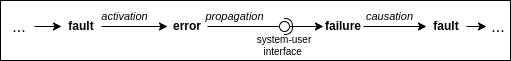
\includegraphics[width=0.95\textwidth]{figures/chapter_2/fault_pathology.drawio.png}
	\caption{The manifestation chain of a fault (\textit{cf.} \cite{concepts_secure_computing}).}
	\label{fig:fault_chain}
\end{figure}

%Catolino \textit{et al.}~\cite{Catolino2019NotAB} use the term bug to classify both development and operational faults in software. Moreover, the authors introduce a taxonomy of common root causes built from reports for software faults, including a class for software faults with security character. 

Faults cause expected scenarios not to run and turn into security faults when they compromise a system's security attributes, \textit{i.e.}, \ac{CIA}. The examples in Figure~\ref{fig:sec_fault_example} depicts the difference. The fault in listing~\ref{bug_ex} does not allow the \textit{pixels} variable to increment. On the other hand, the \textit{security fault} in listing~\ref{vuln_ex} results from wrong bounds-checking the \textit{for} cycle and subjects the system to a memory error. The error can be exploited by loading shell code into the allocated buffer memory, exposing the system to potential malicious use cases. A security fault that is accessible and exploitable is a \textit{vulnerability}. We will elaborate on vulnerabilities in section~\ref{sec:bg_vulns}.
\newline

% ############################## EXAMPLES ########################################
\begin{figure}[!htbp]
    \centering
    \noindent\begin{minipage}{0.48\textwidth}
        % ############################ BUG EXAMPLE ########################################
        \begin{lstlisting}[language = C, numbers = none, escapechar = !, linewidth=0.9\linewidth, basicstyle = \small, backgroundcolor=\color{lightgray}, frame=tb, caption={Fault example (\textit{cf.} \cite{Jason:2000}).}, captionpos=b, label=bug_ex, numbers=left, stepnumber=1]
for (i=0; i<numrows; i++)
    for (j=0; j<numcols; j++)!\textcolor{red}{;}!!\tikz[remember picture] \node [] (a) {};!
        pixels++;
        \end{lstlisting}
    \end{minipage}
    \begin{minipage}{0.45\textwidth}
        % ########################### VULN EXAMPLE ########################################
        \begin{lstlisting}[language = C++, numbers = none, escapechar = !, linewidth=\linewidth, basicstyle = \small, backgroundcolor=\color{lightgray}, frame=tb, caption={Security fault example (\textit{cf.} \cite{Castro:2016}).}, captionpos=b, label=vuln_ex, numbers=left, stepnumber=1] 
void vuln(){
 	int i;
 	int buf[128];
 	
 	for (i=0; !\textcolor{red}{i <= 128}!; i++) !\tikz[remember picture] \node [] (b){};!
 	    cin >> buf[i];
}
        \end{lstlisting}
    \end{minipage}
    \begin{tikzpicture}[remember picture, overlay,
        every edge/.append style = { ->, thick, >=stealth,
                                      darkgray, dashed, line width = 1pt },
        every node/.append style = { align = center, minimum height = 10pt,
                                     font = \bfseries, fill= red!20},
                      text width = 2.5cm ]
      \node [above left = 0.9cm and -0.5cm of a, text width = 2.cm]  (A) {accidental semicolon};
      \node [above left = 1.1cm and 0.5cm of b,text width = 2.cm] (B) {off-by-one error};
      \draw (A.south) + (0.55, 0) coordinate(x1) edge (x1|-a.north);
      \draw (B.south) + (0, 0) coordinate(x1) edge (x1|-b.north);
    \end{tikzpicture}
    \caption{Example of a fault (left) and a security fault (right).}
    \label{fig:sec_fault_example}
\end{figure}

To enforce security policies, Landwehr \textit{et al.}~\cite{taxonomy_security_flaws} characterize security faults by three dimensions: \textit{genesis}, \textit{time of introduction}, and \textit{location}. The former answers how a security fault entered the system and whether it can be \textit{intentional} or \textit{inadvertently}. The time of introduction of a security fault is determined by one of the three different phases in the life cycle of a system: \textit{development}, \textit{maintenance}, or \textit{operational}. For Avizienis \textit{et al.}~\cite{concepts_secure_computing}, the time of introduction resumes with the \textit{development} and \textit{operational} phases, as the latter covers maintenance. During development, all activities up to the release of the initial version of the system can originate security faults, for instance, by including additional mechanisms to the specification for testing the system. During the maintenance phase, activities leading to security faults are often attributable to malicious intrusion or incompetence of the programmer in understanding the system. During the operational phase, unauthorized or unsafe modifications to the system can introduce security faults — \textit{e.g.}, installing virus programs. Finally, a security fault starts manifesting in a location in the system, which can be in the \textit{software} or \textit{hardware}.

Our focus regarding genesis is on accidental security faults as in the latter, the detection approaches are much less likely to help, and measures concern the trustworthiness of the programmers. Regarding the time of introduction and location, our concern is software security faults introduced during the development phase. These can originate in \textit{requirements and specifications}, \textit{source code}, or \textit{object code}. Software requirements and specifications only describe the design of a particular system and its functionality, source code is the actual implementation, and object code only represents the machine-readable form of the previous. We consider source code as we focus on avoiding faults in the software during its implementation to handle threats proactively.

A security fault in software can occur in one of the following software layers: \textit{operating system programs}, \textit{support software}, or \textit{application software}. Similarly, Khwaja \textit{et al.}~\cite{Khwaja2020ASF} identify, based on mitigation techniques, the reach of security faults in software but only at two levels: \textit{operating systems} and \textit{software applications}. Security faults in the former can compromise system functions, such as process and memory management, and cause the most significant injury. Support and application software are programs outside the \ac{OS} boundary — \textit{e.g.}, editors and libraries. Support software has granted privileges, and a security fault in them can allow privilege escalation to gain further unauthorized access to the system. Application software has no special system privileges, but a security fault in them can still cause considerable damage within the storage of the victim. 

\subsection{Classes of Software Security Faults}
\eduard{TODO}
\section{Related Work}
%5.1. Cause-Oriented Taxonomies
%Piessens [139]: Focus on root causes (e.g., data flow errors, logic missteps) to support code review processes.
%Key Points: Categorizes vulnerabilities by “cause families” (e.g., memory mismanagement, faulty authorization).
%Limitation: Primarily addresses code reviewers’ needs; does not account for technology or language context.

%Weber et al. [178]: Taxonomy for code analysis, derived from Landwehr et al.’s OS taxonomy.
%Key Points: Emphasizes vulnerabilities detectable by static code analysis; excludes OS-configuration errors.
%Limitation: Narrow scope—least applicable to high-level application stacks or runtime frameworks.

%5.2. Resource-Oriented Taxonomies
%Bazaz & Arthur [11]: Principal categories based on computable resources: Memory, I/O, Crypto.
%Key Points: Bottom-level taxonomy includes “violable constraints and assumptions” (e.g., buffer sizes).
%Limitation: Resource-centric view can obscure language- or technology-specific patterns (e.g., web frameworks).

%5.3. Susceptibility-Based Taxonomies
%Hughes & Cybenko [77]: NVD-derived eight categories based on a system’s susceptibility (e.g., authentication flaws, data validation).
%Key Points: Data-driven from NVD; correlates categories with prevalence in real CVEs.
%Limitation: Coarse granularity; does not tie back to software type or language.

%5.4. Comprehensive Taxonomy Overviews
%Joshi et al. [82]: Comparative analysis of 25 taxonomies (attack- vs. vulnerability-oriented, OS- vs. software-oriented).
%Key Findings: Only 3/25 are explicitly software-oriented (Piessens [139], Weber [178], Bazaz & Arthur [11]).
%None satisfy all “properties of a good classification” (completeness, mutual exclusivity, etc.). Many are outdated or lack adaptability to modern software ecosystems.

%5.5. Software-Type/Domain-Oriented Taxonomies
%Garg et al. [62]: Classes by software system type (Application, Embedded, OS), severity, technique, and cause.
%Key Findings: 76% of vulnerabilities from 2012–2016 stem from only five vulnerability types; emergent patterns by vendor (e.g., iOS → memory corruption).
%Limitation: Aggregate analyses at a coarse software type; does not examine programming language correlations.

%Tate et al. [167]: Large-scale Linux distro vulnerability classification (Ubuntu, Fedora, SUSE, Debian).
%Key Findings: Out-of-bounds memory access prominently affects kernel and system libraries; logical code design can mitigate detection gaps.

%Ezenwoye et al. [49, 50]: Two complementary studies:

%Ezenwoye et al. [50]: Classify 51,110 NVD entries into seven software types: OS, Browser, Middleware, Utility, Web Application, Framework, Server.
%Findings: Patterns of fault prevalence by software type (e.g., browsers → XSS, servers → configuration issues).

%Ezenwoye et al. [49]: Profile web application faults over ten years by attack method, attack vector, and technology.
%Findings: Web apps most often suffer from injection (SQLi, XSS), cross-site request forgery (CWE-352), and remote file inclusion.


Several studies suggest vulnerability taxonomies oriented toward particular scopes, such as prevalent vulnerability types in specific operating systems~\cite{Tate2020CharacterizingVI}. Joshi \textit{et al.}~\cite{Joshi2015ARO} summarize and compare the characteristics of 25 taxonomies of attacks and vulnerabilities in computer and network systems. Most taxonomies are attack or OS oriented, and only three~\cite{Bazaz2007TowardsAT, Piessens2002ATO, Weber2005ASF} are software oriented. Their analysis indicates that none of the taxonomies satisfy all the necessary principles about classifications. In addition, the existing taxonomies are outdated and limited in use. A standard vulnerability classification method or scheme can increase the security assessment of software systems by providing a common language and a good overview of the field of study. In this section, we offer a summary of the different taxonomies. 

\begin{table}[ht!]
    \centering
    \caption{Summary Table of Reviewed Taxonomies}
    \label{tab:taxonomies-summary}
    \begin{tabular}{l l l l l}
        \hline
        \headcol \textbf{Year} & \textbf{Taxonomy} & \textbf{Scheme} & \textbf{Attributes} & \textbf{Objective} \\
        \hline
        \multirow{2}{*}{1994} & \multirow{2}{*}{Landwehr \textit{et al.}~\cite{taxonomy_security_flaws}} & Multi- & genesis, time, & establish taxonomy of \\
        & & dimensional & location & security faults \\
        \rowcol & & & & understand mistakes\\
        \rowcol \multirow{-2}{*}{2002} & \multirow{-2}{*}{Frank Piessens~\cite{Piessens2002ATO}} & \multirow{-2}{*}{Hierarchical} & \multirow{-2}{*}{genesis, time} & of software developers \\
        \multirow{2}{*}{2005} & \multirow{2}{*}{Weber \textit{et al.}~\cite{Weber2005ASF}} & \multirow{2}{*}{Hierarchical} & \multirow{2}{*}{genesis} & aid designers of code \\
        & & & & analysis tools \\
        \rowcol & & & resources, & strategies to evaluate \\
        \rowcol \multirow{-2}{*}{2007} & \multirow{-2}{*}{Bazaz \& Arthur~\cite{Bazaz2007TowardsAT}} & \multirow{-2}{*}{Hierarchical} & properties & software security \\
        \multirow{2}{*}{2017} & \multirow{2}{*}{Goseva \& Tyo~\cite{GosevaPopstojanova2017SecurityVP}} & Multi- & genesis, severity, & build evidence-based   \\
         & ... & Dimensional & location, time & vulnerability knowledge \\
        \multirow{2}{*}{2019} & \multirow{2}{*}{Garg \textit{et al.}~\cite{Garg2019AnalysisOS}} & Multi- & genesis, severity, &  predictive modeling \& \\
         &  & dimensional & platform, technique &  preemptive mitigation \\
        \multirow{2}{*}{2020} & \multirow{2}{*}{Ezenwoye \textit{et al.}~\cite{Ezenwoye2020ClassifyingCS}} & Single- & \multirow{2}{*}{software type} & reveal prevalence \& \\
         &  & dimensional &  & persistence patterns \\
        ... & ... & ... & ... & ... \\
        \hline
    \end{tabular}
\end{table}

% This is just a categorization from NVD 
% Jeff Hughes and George Cybenko~\cite{Hughes2013QuantitativeMA} categorize vulnerabilities by system susceptibility into eight categories based on the NVD records. 
\par
Frank Piessens~\cite{Piessens2002ATO} proposes a structured taxonomy focusing on the causes of software vulnerabilities to foster the identification of vulnerabilities during software review. Weber \textit{et al.}~\cite{Weber2005ASF} propose a taxonomy of software security faults oriented toward designing code analysis tools. Their taxonomy leverages Landwehr’s work~\cite{taxonomy_security_flaws} and descriptions of vulnerabilities and threats. They re-design the prior classification of security faults by genesis and remove faults not relevant to code analysis tools, such as configuration errors. Anil Bazaz and James Arthur~\cite{Bazaz2007TowardsAT} present a taxonomy of vulnerabilities for assessing software security with verification and validation strategies. Their scheme uses computer resources as the top categories of the taxonomy, covering memory, I/O, and cryptographic resources. The bottom level of the taxonomy conveys violable constraints and assumptions, which allows checking if a software application permits the violation of such constraints and assumptions.
\par
Garg \textit{et al.}~\cite{Garg2019AnalysisOS} classify software vulnerabilities based on software systems, severity level, techniques, and causes. Their classification scheme intends to give a comprehensive view of vulnerabilities in various domains, as vulnerabilities can happen for several reasons in a system. Goseva-Popstojanova and Tyo~\cite{GosevaPopstojanova2017SecurityVP} introduce an empirically driven classification framework that combines CWE-888 Software Fault Pattern (SFP) View with lifecycle phase analysis to create actionable vulnerability profiles. 
% This analysis of recent trends in software vulnerabilities can go somewhere else;  
%The authors also analyze recent trends in software vulnerabilities from 2012–2016 data from the NVD and CVE Details sources. Their analysis indicates that $76\%$ of the total vulnerabilities in the software industry result from only five types of vulnerabilities. It also emerged from the data that few vulnerabilities have a high prominence of affecting specific software systems. For instance, iOS devices are mainly susceptible to \textit{Memory Corruption} vulnerabilities, while Adobe application software is to the \textit{Execution of Code} and \textit{Overflow Memory Corruption}.
% Tate's paper is quite farfetched for the related work
%Tate \textit{et al.}~\cite{Tate2020CharacterizingVI} classify a large set of vulnerabilities in 4 major Linux distributions by the most prevalent vulnerability types. Additionally, the authors examine characteristics of out-of-bounds memory access vulnerabilities and identify that explicit-stated logical design of code can considerably improve the identification of vulnerabilities. 
Ezenwoye \textit{et al.}~\cite{Ezenwoye2020ClassifyingCS} classify 51,110 vulnerability entries from the NVD database into seven software types (OS, browser, middleware, utility, web application, framework, and server). Their analysis demonstrates the pattern of prevalence of software faults by software type. Subsequently, Ezenwoye \textit{et al.}~\cite{Ezenwoye2022WebAW} review ten years of vulnerability data in the NVD database to profile the most common web application faults according to three attributes: attack method, attack vectors, and technology. The latter attribute captures the susceptibility of technologies to faults, including programming languages, frameworks, communication protocols, and data formats. \eduard{there are more recent works that need to be added, e.g., Software Vulnerability Analysis Across Programming Language and Program Representation Landscapes: A Survey}

%\begin{itemize}
%  \item \textbf{Ezenwoye et al. \cite{Ezenwoye2020ClassifyingCS, Ezenwoye2022WebAW}} classify 51,110 CVE entries (2015–2019) by software product type (operating system, browser, middleware, utility, web application, framework, and server). This software-type taxonomy reveals how the prevalence of common weakness categories (such as buffer errors or access-control faults) varies across different platforms, and how certain weakness types persist over time in particular software domains. Their findings provide insights into the vulnerability landscape of each software category.
%  \item \textbf{Garg et al.~\cite{Garg2019AnalysisOS}} propose a holistic taxonomy that links each vulnerability to multiple dimensions simultaneously: the affected software system, the vulnerability’s severity, the exploitation technique, and the root cause of the flaw. By mapping vulnerabilities along these axes, their framework relates each weakness to its context and attributes, enabling a broad, multi-faceted profiling of security faults.
%  \item \textbf{Tate et al.~\cite{Tate2020CharacterizingVI}} perform a longitudinal study of vulnerabilities in a major Linux distribution (Ubuntu) over several years. Analyzing 3,232 security advisories from 2012–2019, they find that out-of-bounds memory access (e.g. classic buffer overflows) consistently dominates the vulnerability profile. Their study identifies trends in vulnerability types over time and examines detailed characteristics of specific exploit instances.  This work underscores the persistent threat of memory-safety errors in open-source Operating System software.
%  \item \textbf{Joshi et al.~\cite{Joshi2015ARO}} review 25 existing taxonomies of attacks and vulnerabilities. They observe that most prior taxonomies focus on attack scenarios or specific platforms (notably operating systems and network protocols). Only a small fraction of the reviewed schemes explicitly target vulnerabilities in the context of general software systems. In other words, Joshi \textit{et al.} find that only a few of the 25 taxonomies are software-oriented, while the majority emphasize attack types or OS-level faults.
%\end{itemize}

\subsection{Identified Gaps}
\eduard{needs to be validated/aligned with the related work above and the gap analysis in the proposal}
Despite these efforts, several important gaps remain:
\begin{itemize}
  \item \textbf{OS- and attack-centric focus:} Existing taxonomies predominantly emphasize operating systems or particular attack vectors (for example, network attacks or web application exploits)~\cite{Joshi2015ARO}.  There is little focus on vulnerabilities specific to application frameworks or general-purpose software contexts.
  \item \textbf{Scarcity of software-oriented taxonomies:} Very few taxonomies (only about 3 of the 25 reviewed by Joshi \textit{et al.}~\cite{Joshi2015ARO}) explicitly classify vulnerabilities by the characteristics of the underlying software system. Most classification schemes do not consider factors such as software architecture, implementation language, or development environment, leaving a gap in understanding vulnerabilities at the application level.
  \item \textbf{Lack of multi-dimensional profiling:} Current classification schemes are largely unidimensional. No existing taxonomy jointly profiles vulnerabilities by intersecting factors (for example, programming language \emph{and} fault type, or software layer and vulnerability cause). This lack of intersectional profiling means we cannot directly relate specific software attributes (such as language or framework) to the kinds of security faults they most frequently exhibit.
  \item \textbf{Absence of unified empirical methods:} There is no single unified, data-driven approach that ties vulnerability records systematically to software characteristics (such as code metrics, library usage, or development practices). Existing approaches either analyze raw CVE data by one attribute (like severity) or propose ad-hoc taxonomies, but none provide an empirical profiling of vulnerabilities linked to software attributes.
\end{itemize}

\subsection{Summary of Research Gap}
In summary, no single comprehensive taxonomy currently exists that profiles software vulnerabilities across multiple levels of granularity and multiple classification dimensions simultaneously.  Existing schemes tend to cover only specific domains or one dimension at a time, leaving gaps in our understanding of how vulnerabilities correlate with software characteristics.  This gap implies that threat modeling and design-time security decisions often lack systematic guidance on which weaknesses are likely in which kinds of software. A more holistic, multi-dimensional vulnerability profiling approach is needed to support effective risk assessment and mitigation. In particular, a unified taxonomy linking vulnerability types to software context and implementation details would enable practitioners to anticipate likely security faults and tailor their prevention strategies across the software development lifecycle~\cite{Joshi2015ARO}.

\section{Methodology} The methodology is structured into three sequential phases, each addressing a distinct part of our multi-dimensional analysis. In Phase I we develop a holistic taxonomy-based representation of security faults. In Phase II we construct an automated data-extraction pipeline to collect and aggregate vulnerability records. In Phase III we perform exploratory analysis on the dataset and derive a hierarchical classification scheme based on observed patterns. Each phase builds on the previous, ensuring a coherent flow from abstract taxonomy to concrete classification.

\subsection{Phase I: Holistic Representation of Security Faults} \textbf{Aim:} Synthesize existing vulnerability taxonomies into a unified attribute schema. This phase consolidates diverse security-fault taxonomies (e.g. language-specific faults, technology categories, architectural layers, and root-cause taxonomies) to create a comprehensive representation of vulnerability attributes.
\newline

%Landwehr’s multi-dimensional foundation: NASA retains genesis (coding errors) and time (phase analysis) but replaces location with subsystem concentration (90% in 2–4 subsystems).

%Piessens’ causal focus: Extends this by linking vulnerability causes to lifecycle phases (e.g., Exception Management flaws stemming from ambiguous error handling during implementation).

%Weber’s tool-oriented schema: Complements by providing empirical data to train static analyzers on NASA’s dominant CWEs (e.g., Risky Values).


\textbf{Steps:}

\begin{itemize}
    \item \textbf{Survey taxonomies.} We collect relevant taxonomies from literature and standards. For example, language- and platform-based taxonomies (e.g. C/C++ errors vs. Web app issues), technology-focused taxonomies (e.g. web, database, OS level), software-layer taxonomies (e.g. presentation vs. business logic), and root-cause taxonomies (e.g. input validation, memory corruption).
    \item \textbf{Identify attributes.} From each taxonomy we extract key attributes (e.g., "Buffer Overflow", "SQL Injection", "Cross-Site Scripting", "Race Condition", etc.) and note which taxonomies include each attribute.
    \item \textbf{Create Unified Attribute Matrix.} We compile these attributes into a matrix with rows as example attributes and columns indicating taxonomy source. Table~\ref{tab:attribute-matrix} (excerpt below) illustrates how attributes map across taxonomies. This "Unified Attribute Matrix" highlights overlaps and gaps, guiding later analysis.
\end{itemize}

\begin{table}[ht!]
    \centering
    \caption{Unified Attribute Matrix}
    \label{tab:attribute-matrix}
    \begin{tabular}{lcccc}
        \hline
        \textbf{Attribute} & \textbf{Lang-based \cite{cwe_list}} & \textbf{Tech-based \cite{Khwaja2020ASF}} & \textbf{Layer \cite{sa_nikolai}} & \textbf{Root Cause \cite{Shahriar2012MitigatingPS}} \\
        \hline
        Buffer Overflow & \checkmark & \checkmark & & \checkmark \\
        SQL Injection & & \checkmark & \checkmark & \\
        Cross-site Scripting & & \checkmark & \checkmark & \\
        Privilege Escalation & \checkmark & & & \checkmark \\
        Invalid Input & & & & \checkmark \\
        \hline
    \end{tabular}
\end{table}

This phase yields a consolidated schema of security fault attributes that will guide data collection and later classification. In particular, the unified list of attributes becomes the basis for labeling and grouping vulnerabilities in subsequent phases.

\subsection{Phase II: Collecting and Analyzing Vulnerability Data} \textbf{Aim:} Gather a large, multi-dimensional vulnerability dataset and compute relevant features for each entry. This involves querying multiple sources (CVE feeds, APIs, repository metadata) and fusing the results into a master dataset for analysis.
\newline
\textbf{Steps:}

\begin{itemize}
    \item \textbf{CVE Data Extraction (get\_cve\_ids\_in\_apps\_with\_cwe.py):} We extract CVE data from the NVD (National Vulnerability Database) JSON feeds using the nvdutils library. We apply specific filtering criteria to focus on:
    \begin{itemize}
        \item Valid CVE entries that affect applications (not operating systems or hardware)
        \item CVEs with associated CWE (Common Weakness Enumeration) identifiers
        \item Selection of the most appropriate CWE ID based on vulnerability mapping, abstraction level, and weakness type
        \item Selection of the most appropriate vulnerable product based on software type and package type
    \end{itemize}
    
    \item \textbf{Product Language Mapping (get\_products\_language.py):} We map software products to their programming languages using:
    \begin{itemize}
        \item Package URL (purl) to CPE mappings from a SQLite database
        \item Predefined mappings of package types to languages (e.g., maven → Java, pypi → Python)
        \item GitHub API queries to determine the primary language of repositories
    \end{itemize}
    
    \item \textbf{Software Type Categorization (get\_software\_type.py):} We categorize software products into different types (e.g., extension, package, mobile\_app, framework, utility, server, web\_application) based on:
    \begin{itemize}
        \item The official CPE dictionary from NVD
        \item A research dataset from a published paper
        \item Product name analysis using predefined keywords
    \end{itemize}
    
    \item \textbf{Dataset consolidation:} We merge all gathered information into a unified table. Each row corresponds to one vulnerability and includes attributes such as CVE ID, CWE ID, vendor, product, programming language, and software type. To have more accurate information on the programming language, we employ a text analysis approach to extract language information from CVE descriptions by:
    \begin{itemize}
        \item Identifying file names with known extensions mentioned in vulnerability descriptions
        \item Mapping these file extensions to their corresponding programming languages
        \item Determining the most likely language based on the frequency of file extensions
    \end{itemize}

\end{itemize}


Figure~\ref{fig:pipeline} schematically depicts the data extraction pipeline, and Table~\ref{tab:vuln-dataset} shows sample rows from the final dataset. These integrations leverage multiple tools and APIs to maximize coverage of relevant fields. 
Figure~\ref{fig:extraction-pipeline} (above) illustrates the multi-stage data pipeline used in Phase II. We automatically download the NVD CVE feeds, augment records via the CVE Details API, query GitHub for project context, and apply purl2cpe translation, ultimately producing a consolidated CSV dataset. 

\begin{table}[h!]
\centering
\caption{Example rows from vuln\_master\_dataset.csv after data collection. Each entry includes CVE ID, project context, CWE class, and a brief description.}
\label{tab:vuln-dataset}
\begin{tabular}{llllp{4cm}}
\hline
\textbf{CVE} & \textbf{Project} & \textbf{CWE} & \textbf{Severity} & \textbf{Short Description} \\
\hline
CVE-2021-12345 & ProjectA & CWE-79 (XSS) & High & Stored XSS in user comments widget \\
CVE-2020-67890 & ProjectB & CWE-89 (SQLi) & Medium & SQL injection in search query builder \\
CVE-2019-11111 & ProjectC & CWE-119 (Overflow) & Critical & Buffer overflow in image parser \\
... & ... & ... & ... & ... \\
\hline
\end{tabular}
\end{table}

We include citations to the APIs and data sources used: NVD/CVE as in~\cite{nvd_nist}, the CVE Details service~\cite{cve_details}, the GitHub REST API, and the purl2cpe resource~\eduard{add/fix references}. Each component is validated to ensure accurate parsing and merging of fields.

\subsection{Phase III: Mapping Analysis Results to Classification Scheme} \textbf{Aim:} Analyze the collected data to identify recurring patterns and design a multi-level classification scheme for security faults. The goal is to move from raw data to insight, culminating in a hierarchical taxonomy (Dimension $\rightarrow$ Subclass $\rightarrow$ Example CWE) that reflects the observed diversity of vulnerabilities.
\newline

\textbf{Steps:}
\begin{itemize}
    \item \textbf{Exploratory Analysis.} We perform statistical and visual analyses on the dataset. This includes generating histograms of vulnerabilities by language, technology, and layer; heatmaps showing co-occurrence of attributes; and scatter plots for correlations (e.g. severity vs. time). These visuals help highlight the most prominent fault attributes and gaps.
    \item \textbf{Pattern extraction.} From the visualizations we identify recurring themes. For instance, we may observe that web-related vulnerabilities (CWE-79, CWE-89) cluster in the "Technology: Web" category, or that certain root causes (e.g. improper input validation, CWE-20) appear across multiple languages and frameworks.
    \item \textbf{Classification hierarchy design.} Guided by the unified attributes (from Phase I) and patterns, we construct a three-level classification. The top level ("Dimension") corresponds to our major analysis axes (e.g. {\em Programming Language}, {\em Technology Domain}, {\em Architectural Layer}, {\em Root Cause}). The second level ("Subclass") refines each dimension (e.g. for Language: {\em Web Languages} vs. {\em System Languages}). The third level lists concrete examples, typically specific CWE identifiers or vulnerability types (e.g. {\em CWE-79: XSS} under "Technology: Web"). An excerpt of this hierarchy is shown in Table~\ref{tab:classification}, and its conceptual organization is visualized in Figure~\ref{fig:classification-hierarchy}.
\end{itemize}

\begin{table}[h!]
\centering
\caption{Excerpt of the classification hierarchy (Phase III): Dimension $\rightarrow$ Subclass $\rightarrow$ Example CWE.}
\label{tab:classification}
\begin{tabular}{lll}
\hline
\textbf{Dimension} & \textbf{Subclass} & \textbf{Example CWE} \\
\hline
Language & Web-facing languages & CWE-79 (Cross-site scripting) \\
Language & System languages & CWE-120 (Buffer overflow) \\
Technology & Web frameworks & CWE-89 (SQL injection) \\
Technology & Mobile applications & CWE-22 (Path traversal) \\
Layer & Network layer & CWE-319 (Cleartext transfer) \\
Layer & Application layer & CWE-416 (Use-after-free) \\
Root Cause & Input validation errors & CWE-20 (Improper input check) \\
Root Cause & Memory management errors & CWE-119 (Buffer overflow) \\
\hline
\end{tabular}
\end{table}


\begin{figure}[!h]
	\centering
    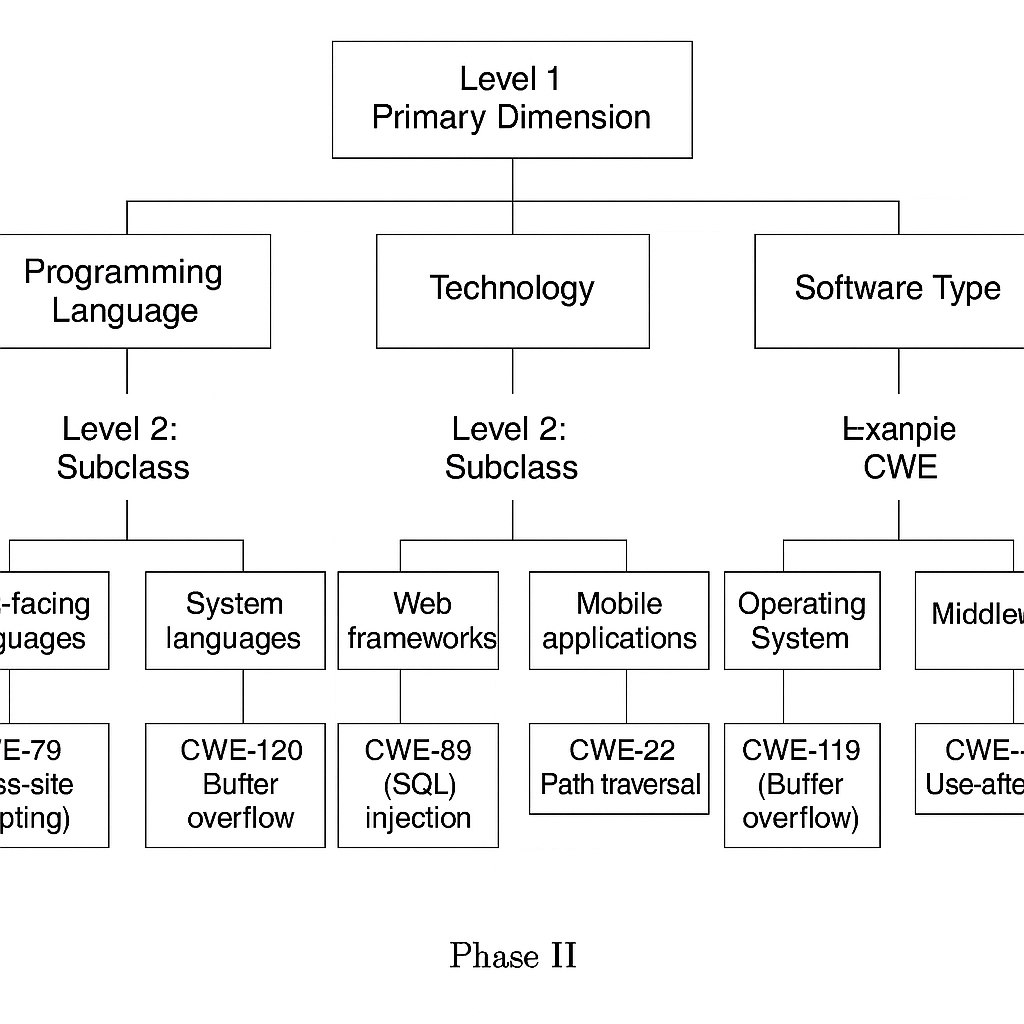
\includegraphics[width=0.55\textwidth]{figures/chapter_2/classification-hierarchy.png}
	\caption{Hierarchical classification}
	\label{fig:classification-hierarchy}
\end{figure}


Figure~\ref{fig:classification-hierarchy} (above) sketches the hierarchical classification derived in Phase III. Each Dimension branches into subclasses with illustrative CWE examples at the leaves. This taxonomy is rooted in the empirical data patterns uncovered and in prior taxonomies cited earlier. Through these steps, Phase III links the aggregated data back to our taxonomy framework, revealing how software vulnerabilities distribute across the multi-dimensional space. The resulting classification scheme provides a structured way to profile security faults, based both on existing knowledge (the taxonomies) and new insights from the data analysis.
\section{Results}

Our analysis of the National Vulnerability Database (NVD) yielded a comprehensive dataset that allows us to profile security faults across multiple dimensions. Following the methodology outlined in Phase II, we present the results of our data collection and analysis, addressing the research question of how software security faults profile regarding software type, technology, causes, and programming language.

\subsection{How do vulnerability patterns differ across software types?}

To understand how vulnerability patterns vary by software type, we analyzed the 100\%‐stacked distribution of the top CWEs across seven categories of software products (extension, framework, library, mobile\_app, server, utility, web\_application). This analysis builds on the consolidated dataset of 55,657 CVEs for which software type was determined, after mapping products to types and programming languages as described in the methodology.

Figure~\ref{fig:sw_typ_cwe} (100\%‐stacked bar chart) shows the relative frequency of four prominent CWEs (CWE-352: Cross-Site Request Forgery; CWE-787: Out-of-Bounds Write; CWE-79: Cross-Site Scripting; CWE-89: SQL Injection) along with “Others” (all remaining CWEs) for each software type. The key observations are as follows:

\begin{figure}[!h]
	\centering
    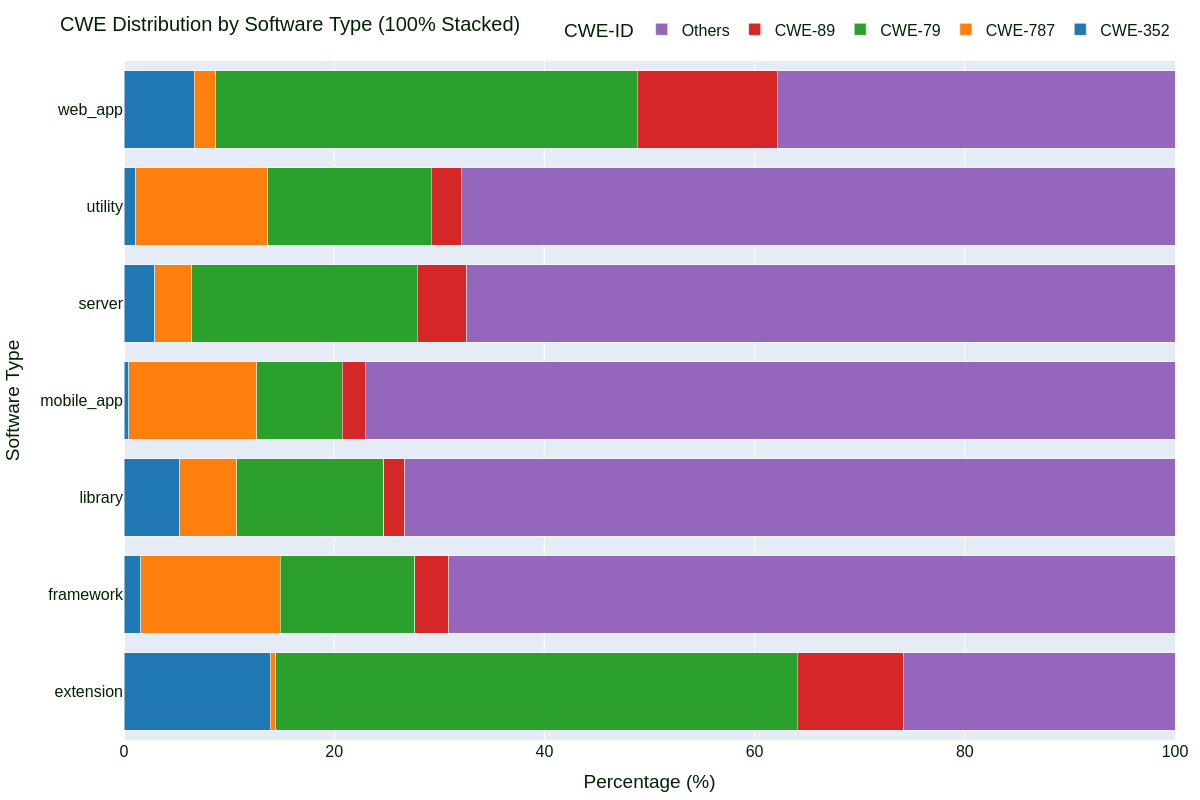
\includegraphics[width=0.95\textwidth]{figures/chapter_2/stacked_bar_software_cwe.png}
	\caption{100\%‐stacked bar chart of CWE Distribution by Software Type}
	\label{fig:sw_typ_cwe}
\end{figure}

\begin{itemize}
    \item \textbf{Extensions}: Nearly half of the vulnerabilities in extensions are XSS (CWE-79: 49.6\%), followed by CSRF (CWE-352: 13.9\%) and SQL Injection (CWE-89: 10.2\%), with a substantial residual portion (25.8\%) in “Others.” This suggests that browser or plugin-like components are predominantly exposed to web-based injection and script injection flaws, likely due to their frequent interaction with untrusted web content or APIs.
    \item \textbf{Web Applications}: Web applications similarly exhibit a high proportion of XSS (40.1\%) and SQL Injection (13.3\%), with CSRF accounting for 6.7\% and “Others” comprising 37.9\%. This aligns with expectations for web-facing services, where input validation and session/state management issues are primary concerns.
    \item \textbf{Servers}: Server software shows a moderate share of XSS (21.5\%) and lower SQL Injection (4.7\%) and CSRF (2.9\%), with “Others” at 67.4\%. The lower injection percentages may reflect that many server-side components rely on different interfaces (e.g., APIs, network protocols) where other types of weaknesses (captured in “Others”) predominate.
    \item \textbf{Frameworks}: Frameworks stand out with a notable portion of memory-related issues (CWE-787: 13.3\%), alongside XSS (12.8\%) and a large “Others” category (69.1\%). This indicates that underlying libraries or platforms (e.g., web frameworks, application frameworks) face both input-handling flaws and lower-level implementation bugs, including memory safety vulnerabilities.
    \item \textbf{Libraries}: Libraries have a smaller fraction of XSS (14.0\%) and Out-of-Bounds Write (5.4\%), with most vulnerabilities falling into “Others” (73.3\%). This diffuse distribution suggests libraries span a wide range of functionality, so specific weakness patterns vary greatly depending on the domain (e.g., cryptography, data processing, image handling).
    \item \textbf{Utilities}: Utility software shows a moderate XSS share (15.6\%) and a higher proportion of Out-of-Bounds Write (12.5\%), with “Others” at 67.9\%. Utilities (e.g., command-line tools, system utilities) often involve file or memory operations, which may explain the relative prominence of memory-related flaws alongside occasional script or injection issues when utilities process complex inputs.
    \item \textbf{Mobile Applications}: Mobile apps exhibit a small fraction of XSS (8.1\%) but a notable Out-of-Bounds Write share (12.2\%), with “Others” dominating (77.0\%). This pattern reflects that while mobile apps may embed webviews (leading to some XSS), many vulnerabilities arise from platform-specific memory handling or misuse of APIs.
\end{itemize}

Overall, software types with strong web-facing components (extensions, web applications) show high proportions of injection and scripting weaknesses, whereas types closer to system-level or framework-level code (frameworks, utilities, mobile apps) surface more memory-related issues. Libraries cover a broad spectrum, resulting in a large “Others” bucket. Servers lie in between, with diverse vulnerabilities but fewer classical web injection flaws.

\begin{boxC}
\textit{\textbf{Finding 1.} Vulnerability patterns vary significantly by software type: web-facing contexts (extensions, web applications) are dominated by script- and injection-related weaknesses (e.g., XSS, SQL Injection), while frameworks, utilities, and mobile applications exhibit higher rates of memory safety issues (e.g., out-of-bounds writes). Libraries show diffuse patterns across many weakness types. This implies that security mitigations should be tailored to software type, emphasizing input validation and sanitization for web components, and memory safety practices for frameworks and system-oriented software.}
\end{boxC}

\subsection{How do programming languages correlate with security faults?}

Our language mapping process successfully identified the primary programming language for 13,081 vulnerable software products. The distribution reveals several key insights:

\begin{itemize}
    \item Web-oriented languages dominate the vulnerability landscape, with PHP (32.4\%, 4,236 samples) and JavaScript (13.9\%, 1,824 samples) accounting for nearly half of all identified vulnerabilities.
    \item Java (10.8\%, 1,415 samples) represents a significant portion, reflecting its widespread use in enterprise applications.
    \item Systems programming languages like C (6.8\%, 887 samples) and C++ (3.4\%, 448 samples) show fewer vulnerabilities in absolute numbers but may represent more severe issues when they occur.
    \item Modern languages like Python (6.2\%, 817 samples), Go (3.8\%, 496 samples), and Rust (2.0\%, 267 samples) are present but with lower frequency, potentially indicating better security properties or less widespread adoption.
\end{itemize}

The predominance of PHP and JavaScript vulnerabilities aligns with their extensive use in web development, where exposure to user input creates numerous attack vectors. The relatively lower representation of systems languages may reflect either better security practices or the challenges in vulnerability discovery for these languages.

\subsection{Common Weakness Enumeration (CWE) Analysis}

Our analysis extracted 18,566 CVE entries with associated CWE identifiers, revealing the most common vulnerability types:

\begin{itemize}
    \item Cross-Site Scripting (CWE-79) dominates with 32.3\% (6,000 samples) of all vulnerabilities, highlighting the persistent challenge of securing user input in web applications.
    \item Cross-Site Request Forgery (CWE-352, 7.7\%, 1,434 samples) and SQL Injection (CWE-89, 7.1\%, 1,316 samples) represent the next tier of common web vulnerabilities.
    \item Path Traversal (CWE-22, 4.8\%, 899 samples) and Authorization Issues (CWE-862, 3.9\%, 727 samples) round out the top five.
    \item Memory corruption vulnerabilities like Out-of-bounds Write (CWE-787, 3.6\%, 661 samples) and Out-of-bounds Read (CWE-125, 2.3\%, 422 samples) appear less frequently but often represent higher severity issues.
\end{itemize}

The prevalence of web-related vulnerabilities (CWE-79, CWE-352, CWE-89) reflects the extensive attack surface of web applications and the challenges in properly validating and sanitizing user input. Memory corruption vulnerabilities, while less common, remain a persistent threat, particularly in systems programming contexts.

\subsection{Multi-dimensional Vulnerability Profiling}

The consolidated dataset (18,566 samples total, including 7,868 products with both language and software type identified) reveals important patterns across software types, programming languages, and vulnerability classes:

\begin{itemize}
    \item PHP-based extensions and web applications are particularly susceptible to Cross-Site Scripting (CWE-79), with 2,175 and 1,450 instances respectively, representing the most common vulnerability profiles.
    \item Cross-Site Request Forgery (CWE-352) is also prevalent in PHP extensions (607 instances) and web applications (334 instances).
    \item SQL Injection (CWE-89) affects PHP web applications (477 instances) and extensions (399 instances) most frequently.
    \item JavaScript applications show significant vulnerability to Cross-Site Scripting (CWE-79, 245 instances), while Java libraries exhibit both XSS (221 instances) and CSRF (188 instances) vulnerabilities.
    \item Memory corruption vulnerabilities cluster in C-based frameworks (CWE-787, 158 instances; CWE-125, 147 instances) and utilities (CWE-125, 154 instances; CWE-787, 138 instances).
\end{itemize}

These patterns reveal distinct vulnerability profiles across the software ecosystem:

\begin{enumerate}
    \item \textbf{Web Application Profile:} Dominated by input validation vulnerabilities (XSS, CSRF, SQLi) in PHP and JavaScript applications, particularly in extensions and web applications.
    \item \textbf{Systems Software Profile:} Characterized by memory corruption issues (buffer overflows, use-after-free) in C and C++ utilities and frameworks.
    \item \textbf{Enterprise Application Profile:} Represented by a mix of web vulnerabilities and authorization issues in Java libraries and frameworks.
\end{enumerate}

\subsection{Addressing the Research Question}

Returning to our research question—\textit{How do software security faults profile regarding software type, technology, causes, and programming language?}—our analysis reveals several key insights:

\begin{itemize}
    \item \textbf{Software Type:} Extensions and web applications are most vulnerable to input validation issues, while utilities and frameworks show greater susceptibility to memory corruption. Servers exhibit a more diverse vulnerability profile spanning both categories.

    \item \textbf{Technology:} Web technologies dominate the vulnerability landscape, with client-side (XSS, CSRF) and server-side (SQLi, path traversal) issues being most prevalent.

    \item \textbf{Causes:} Improper input validation emerges as the dominant root cause across the ecosystem, followed by memory management issues in systems software and authorization problems across multiple software types.

    \item \textbf{Programming Language:} Strong correlations exist between languages and vulnerability types: PHP and JavaScript with web vulnerabilities, C and C++ with memory corruption, and Java with a mix of web and authorization issues.
\end{itemize}

These findings demonstrate that vulnerability profiles are not uniform across the software ecosystem but rather cluster into distinct patterns based on software type, implementation language, and application domain. This multi-dimensional profiling provides a more nuanced understanding of security fault distribution than previous single-dimensional analyses.

\section{Discussion}
\eduard{TODO}

\section{Threats to Validity}

In this section, we discuss potential threats to the validity of our study, categorized into four main types: internal validity, external validity, construct validity, and conclusion validity.

\subsection{Internal Validity}

Internal validity concerns the extent to which our methodology allows for accurate causal inferences.

\begin{itemize}
    \item \textbf{Data extraction accuracy:} The automated data extraction process may introduce errors or inconsistencies. While we implemented validation checks, the complexity of parsing and merging data from multiple sources could lead to inaccuracies in the final dataset.

    \item \textbf{Selection bias in CWE mapping:} Our algorithm for selecting the "most appropriate" CWE ID for each vulnerability involves prioritization based on vulnerability mapping, abstraction level, and weakness type. This selection process may introduce bias by favoring certain types of weaknesses over others.

    \item \textbf{Temporal effects:} The NVD database is continuously updated, with both new vulnerabilities being added and existing entries being modified. Our analysis represents a snapshot at a specific point in time, which may affect the stability of our findings.
\end{itemize}

\subsection{External Validity}

External validity concerns the generalizability of our findings to other contexts.

\begin{itemize}
    \item \textbf{Representativeness of the sample:} While the NVD is a comprehensive database, it may over-represent certain types of software or vulnerabilities. For example, open-source projects may be more likely to have their vulnerabilities reported and documented compared to proprietary software.

    \item \textbf{Technological evolution:} The rapid evolution of technology means that the patterns and distributions of vulnerabilities observed in our study may not generalize to future software systems or emerging technologies.
\end{itemize}

\subsection{Construct Validity}

Construct validity concerns whether we are measuring what we intend to measure.

\begin{itemize}
    \item \textbf{Language classification:} Our classification of programming languages into primary (general-purpose) and secondary (domain-specific) categories may not capture the full complexity of language ecosystems. Some languages may span multiple categories or evolve over time.

    \item \textbf{Software type categorization:} The categorization of software into different types based on predefined mappings and keyword analysis may not always accurately reflect the true nature or purpose of the software.

    \item \textbf{CWE abstraction levels:} The CWE hierarchy includes different levels of abstraction (e.g., Class, Base, Variant). Our preference for more specific abstractions may not always align with how vulnerabilities are conceptualized in practice.
\end{itemize}

\subsection{Conclusion Validity}

Conclusion validity concerns the reliability of our conclusions based on the data and analysis.

\begin{itemize}
    \item \textbf{Pattern identification:} The identification of patterns in the exploratory analysis phase relies on visual inspection and statistical methods. There is a risk of identifying spurious patterns or missing significant but subtle relationships.

    \item \textbf{Classification hierarchy design:} The design of our three-level classification hierarchy (Dimension → Subclass → Example CWE) involves subjective decisions about how to organize and categorize vulnerabilities. Different researchers might arrive at different classification schemes given the same data.

    \item \textbf{Interpretation of results:} The interpretation of the relationships between software types, programming languages, and CWEs may be influenced by preconceptions or biases in how we understand and categorize security vulnerabilities.
\end{itemize}

To mitigate these threats, we have implemented several measures, including validation checks in our data extraction pipeline, cross-referencing multiple data sources, and using established taxonomies as a foundation for our classification scheme. We also acknowledge that our findings should be interpreted within the context of these limitations and that further research is needed to validate and extend our results.

\section{Summary}
\eduard{TODO}




%%----------------------------------------
%% Final materials
%%----------------------------------------

%% Bibliography
\PrintBib

%% comment next 2 commands if numbered appendices are not used
%\appendix
%%% an example of appendix
\chapter{Lorem Ipsum} \label{ap1:Lorem}

After the conclusions and bibliographical references,
the text used to complete the dissertation is presented in this 
numbered annex. 

\section{What is \emph{Lorem Ipsum}?}

\emph{\textbf{Lorem Ipsum}} is simply dummy text of the printing and
typesetting industry. Lorem Ipsum has been the industry's standard
dummy text ever since the 1500s, when an unknown printer took a galley
of type and scrambled it to make a type specimen book. It has survived
not only five centuries, but also the leap into electronic
typesetting, remaining essentially unchanged. It was popularised in
the 1960s with the release of Letraset sheets containing Lorem Ipsum
passages, and more recently with desktop publishing software like
Aldus PageMaker including versions of Lorem Ipsum~\cite{kn:Lip08}. 

\section{Where does \emph{Lorem} come from?}

Contrary to popular belief, Lorem Ipsum is not simply random text. It
has roots in a piece of classical Latin literature from 45 BC, making
it over 2000 years old. Richard McClintock, a Latin professor at
Hampden-Sydney College in Virginia, looked up one of the more obscure
Latin words, consectetur, from a Lorem Ipsum passage, and going
through the cites of the word in classical literature, discovered the
undoubtable source. Lorem Ipsum comes from sections 1.10.32 and
1.10.33 of ``de Finibus Bonorum et Malorum'' (The Extremes of Good and
Evil) by Cicero, written in 45 BC. This book is a treatise on the
theory of ethics, very popular during the Renaissance. The first line
of Lorem Ipsum, ``Lorem ipsum dolor sit amet\ldots'', comes from a line in
section 1.10.32.

The standard chunk of Lorem Ipsum used since the 1500s is reproduced
below for those interested. Sections 1.10.32 and 1.10.33 from ``de
Finibus Bonorum et Malorum'' by Cicero are also reproduced in their
exact original form, accompanied by English versions from the 1914
translation by H. Rackham.

\section{Why is \emph{Lorem} used?}

It is a long established fact that a reader will be distracted by the
readable content of a page when looking at its layout. The point of
using Lorem Ipsum is that it has a more-or-less normal distribution of
letters, as opposed to using ``Content here, content here'', making it
look like readable English. Many desktop publishing packages and web
page editors now use Lorem Ipsum as their default model text, and a
search for ``lorem ipsum'' will uncover many web sites still in their
infancy. Various versions have evolved over the years, sometimes by
accident, sometimes on purpose (injected humour and the like). 

\section{Where can you find examples?}

There are many variations of passages of Lorem Ipsum available, but
the majority have suffered alteration in some form, by injected
humour, or randomised words which don't look even slightly
believable. If you are going to use a passage of Lorem Ipsum, you need
to be sure there isn't anything embarrassing hidden in the middle of
text. All the Lorem Ipsum generators on the Internet tend to repeat
predefined chunks as necessary, making this the first true generator
on the Internet. It uses a dictionary of over 200 Latin words,
combined with a handful of model sentence structures, to generate
Lorem Ipsum which looks reasonable. The generated Lorem Ipsum is
therefore always free from repetition, injected humour, or
non-characteristic words etc. 


\end{document}
